% mainfile: ../../../../master.tex
\subsection{Quantification with Qubit\texttrademark~ RNA BR Assay}
% The part of the label after the colon must match the file name. Otherwise,
% conditional compilation based on task labels does NOT work.
\label{task:20180215_cj2}
\tags{lab,qnt,rna}
\authors{cj}
%\files{}
%\persons{}

I basically did the same with the RNA sample as I did for the DNA. I used the same samples twice with different input volumes for the assay. And I repeated the measurement (including calibration) twice.

\begin{figure}[H] % position of the figure 
    \centering
    \caption{Illustration for the Qubit\texttrademark~ RNA BR assay}
    \label{fig:20180215_Qubit_RNA_BR}
    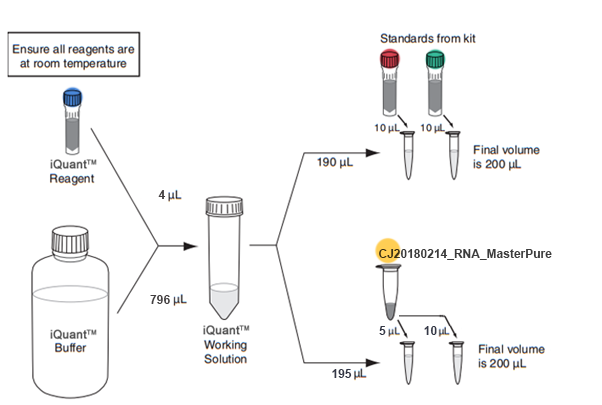
\includegraphics[width=0.8\textwidth]{graphics/schemas/20180215_Qubit_RNA_BR.png}
\end{figure}

\begin{table}[H]
\caption{Total RNA quantities in samples measured with Qubit\texttrademark~ RNA BR Assay Kit}
\label{tab:20180215_rna_qnt}
\centering
\begin{tabular}{l r r r r}
\toprule
Sample ID & \textmu g/mL & $V_f$ (mL) & m (\textmu g) & m (ng) \\ \midrule
\texttt{CJ20180214\_RNA\_MasterPure\_5} & 32.8 & 0.033 & 1.08 &  1082.4 \\
\texttt{CJ20180214\_RNA\_MasterPure\_10} & 32.6 & 0.033 & 1.072 &1072.5 \\
\texttt{CJ20180214\_RNA\_MasterPure\_5} & 32.6 & 0.033 & 1.072 & 1072.5 \\
\texttt{CJ20180214\_RNA\_MasterPure\_10} & 32.2 & 0.033 & 1.062 & 1062.6 \\
\bottomrule
\end{tabular}
\end{table}

According these measurments, I have currently -- at least -- 1~\textmu g of RNA. But initially (before quantifications) I had 1.61~\textmu g of RNA. Knowing that this is the yield from 4~mL of micro-algae cultures, I hope to be able to retrieve even more nucleic acids from few liters of seawater.

The next step is to reverse transcribe these RNA samples (extracted with MasterPure\texttrademark~ and AllPrep) and then to amplify both cDNA and extracted DNA to see the contaminants are not inhibiting the downstream processes.





